%!TEX program = xelatex
\documentclass[11pt]{article}
\usepackage{amsmath,amssymb,amsthm}
\usepackage{filecontents}
\usepackage{graphicx}
\usepackage{tikz}


\DeclareMathOperator*{\xE}{\mathbb{E}}
\let\Pr\relax
\DeclareMathOperator*{\Pr}{\mathbb{P}}

\newcommand{\eps}{\varepsilon}
\newcommand{\inprod}[1]{\left\langle #1 \right\rangle}
\newcommand{\R}{\mathbb{R}}

\newcommand{\handout}[5]{
  \noindent
  \begin{center}
  \framebox{
    \vbox{
      \hbox to 5.78in { {\bf CS 121: Introduction to Theoretical Computer Science } \hfill #2 }
      \vspace{4mm}
      \hbox to 5.78in { {\Large \hfill #5  \hfill} }
      \vspace{2mm}
      \hbox to 5.78in { {\em #3 \hfill #4} }
    }
  }
  \end{center}
  \vspace*{4mm}
}

\newcommand{\lecture}[4]{\handout{#1}{#2}{#3}{#4}{Section #1}}

\newtheorem{theorem}{Theorem}
\newtheorem*{proposition}{Proposition}
\newtheorem{lemma}[theorem]{Lemma}
\newtheorem{corollary}[theorem]{Corollary}
\newtheorem{conjecture}[theorem]{Conjecture}
\newtheorem{postulate}[theorem]{Postulate}
\theoremstyle{definition}
\newtheorem{defn}[theorem]{Definition}
\newtheorem{example}[theorem]{Example}

\theoremstyle{remark}
\newtheorem*{remark}{Remark}
\newtheorem*{notation}{Notation}
\newtheorem*{note}{Note}

% \DeclareUnicodeCharacter{1F346}{\eggplant}

\newcommand{\sub}{\operatorname{sub}}
\newcommand{\quot}{\operatorname{quot}}
\newcommand{\bw}{\bigwedge}
\newcommand{\Avs}{\operatorname{Av}^{\operatorname{sign}}}
\newcommand{\bad}{\operatorname{bad}}
\newcommand{\sign}{\operatorname{sign}}
\newcommand{\id}{\operatorname{id}}
\newcommand{\defeq}{\vcentcolon=}
\newcommand{\eqdef}{=\vcentcolon}
%We can even define a new command for \newcommand!
\newcommand{\nc}{\newcommand}
\nc{\on}{\operatorname}
\nc\renc{\renewcommand}
\nc{\BR}{\mathbb R}
\nc{\BG}{\mathbb G}
\nc{\BP}{\mathbb P}
\nc{\BC}{\mathbb C}
\nc{\BQ}{\mathbb Q}
\nc{\BF}{\mathbb F}
\nc{\BZ}{\mathbb Z}
\nc{\BN}{\mathbb N}
\nc{\BS}{\mathbb S}
\nc{\Hom}{\on{Hom}}
\nc{\wt}{\widetilde}
\nc{\vspan}{\on{span}}
\nc{\ord}{\on{ord}}
\nc{\im}{\on{im}}
\nc{\Mat}{\on{Mat}}
\nc{\can}{\on{can}}
\nc{\coker}{\on{coker}}
\nc{\ev}{\on{ev}}
\nc{\Tr}{\on{Tr}}
\nc{\End}{\on{End}}
\nc{\swap}{\on{swap}}
\nc{\Set}{\on{Set}}
\nc{\bC}{{\mathbf C}}
\nc{\bc}{{\mathbf c}}
\nc{\bD}{{\mathbf D}}
\nc{\bd}{{\mathbf d}}
\nc{\bE}{{\mathbf E}}
\nc{\be}{{\mathbf e}}
\nc{\bF}{{\mathbf F}}
\nc{\bff}{{\mathbf f}}
\nc{\CE}{\mathcal E}
\nc{\CD}{\mathcal D}
\nc{\CH}{\mathcal H}
\nc{\CY}{\mathcal Y}
\renc{\mod}{\on{-mod}} %Careful - turn this off in a number theory setting
\newcommand{\spec}{\text{spec}}
\nc{\adj}{\on{adj}}
\nc{\tensor}[3]{#1 \underset{#2}\otimes #3}
\nc{\Nat}{\on{Nat}}
\nc{\op}{\on{op}}
\nc{\Funct}{\on{Funct}}
\nc{\Ob}{\on{Ob}}
\nc{\fR}{\mathfrak{R}}
\nc{\Vect}{\on{Vect}}
\nc{\ns}{\on{non-spec}}
\nc{\ol}{\overline}
\nc{\ul}{\underline}
\nc{\univ}{\on{univ}}
\nc{\Maps}{\on{Maps}}
\nc{\bdd}{\on{bdd}}
\nc{\cont}{\on{cont}}
\nc{\Sym}{\on{Sym}}
\nc{\vol}{\on{vol}}
\nc{\supp}{\on{supp}}
\nc{\Lie}{\on{Lie}}
\nc{\master}{\on{master}}
\nc{\pt}{\on{pt}}
% \nc{\dim}{\on{dim}}

\nc{\dy}{\on{dy}}

\providecommand{\tightlist}{%
  \setlength{\itemsep}{0pt}\setlength{\parskip}{0pt}}


% 1-inch margins, from fullpage.sty by H.Partl, Version 2, Dec. 15, 1988.
\topmargin 0pt
\advance \topmargin by -\headheight
\advance \topmargin by -\headsep
\textheight 8.9in
\oddsidemargin 0pt
\evensidemargin \oddsidemargin
\marginparwidth 0.5in
\textwidth 6.5in

\parindent 0in
\parskip 1.5ex

\usepackage{natbib}

\begin{document}
% Change these parameters accordingly!
\nc{\sectionnumber}{6}
\nc{\thedate}{}
\nc{\tfnames}{}


\lecture{\sectionnumber}{Fall 2019}{Prof.\ Boaz Barak}{\tfnames}

% Cover lectures 7/8

% Relevant lecture notes:
% https://files.boazbarak.org/introtcs/lec_06_loops.pdf
% https://files.boazbarak.org/introtcs/lec_07_other_models.pdf

% Potentially relevant old section notes:
% https://github.com/boazbk/cs121fall2019/tree/master/2018_material/sections/section_3
% https://github.com/boazbk/cs121fall2019/tree/master/2018_material/sections/section_4
% https://github.com/boazbk/cs121fall2019/blob/master/2018_material/sections_2018/section_2/section_2
% https://github.com/boazbk/cs121fall2019/tree/master/2018_material/sections_2018/section_3


\section{Efficient Algorithms}

\noindent We have spent much of the semester asking \textit{if} something is computable or not.
Now we ask: how long or how many resources does a computation take? One difference we are particular concerned with is the difference between \textbf{polynomial} and \textbf{exponential} running time, which we will formally define later.

\subsection{Min Path/Max Path}

\noindent Recall that a graph $G$ has a set $V$ of $n$ vertices and a set $E$ of
$m$ edges. 

\begin{itemize}
    \item \textsf{MINPATH}: On input a triple $(G, s, t)$, output the number $k$ which is the length of the shortest path between $s$ and $t$, or $-1$ if no such path exists.
    Using BFS, can be computed in $O(n+m)$ time, which is $O(m)$ since $m \geq n-1.$ This is \textbf{polynomial} time.
    
    \item \textsf{MAXPATH}: Given $(G, s, t)$, find the longest non-intersecting path between $s$ and $t$.
    The best algorithm takes \textbf{exponential} time.
    
\end{itemize}


\subsection{Min Cut/Max Cut}
We define a cut in a graph, $G = (V, E)$ as follows. Given a graph $G=(V, E)$, a \textit{cut} is a subset of $S$ of $V$ such that $S$ is neither empty nor all of $V$. The edges cut by $S$ are those edges where one of their endpoints is in $S$ and the other is in $\overline{S}=V \setminus S.$ If $s, t \in V$, an $s, t$ cut is a cut such that $s \in S, t \in \overline{S}.$

\begin{itemize}
\item The \textsf{MINPATH} problem is the problem of finding the minimum $s, t$ cut. More formally: Given $(G, s, t)$, find the minimum number $k$ such that there is an $s, t$ cut cutting $k$ edges (i.e. there exists a set $S$ containing $s$ and not $t$ with exactly $k$ edges that touch $S$ and $\overline{S}.$) There exists an algorithm, the Edmonds-Carp algorithm, that can find the minimum cut between two nodes in $O(n\cdot m^2)$ time: \textbf{polynomial} running time. 

\item The \textsf{MAXCUT} problem however trying to find the maximum $k$ takes \textbf{exponential} time, and is the brute-force algorithm that tries all $2^n$ possibilities for $S$.

\end{itemize}


\noindent \textbf{Exercise:} How can we use the Edmonds-Carp algorithm as a black-box to find the minimum cut between any nodes in the graph? What is the time complexity?\\

\noindent \textbf{Solution:} There are $n \choose 2$ pairs of nodes in the graph. We could run Edmonds-Carp on all $\frac{n(n-1)}{2}$ pairs, and take the minimum over all pairs. This would have a total time complexity of $O(n^3m^2)$, which is polynomial.


\subsection{Existence of a $k$-clique}

\noindent Checking for the existence of $k$-clique is polynomial time for a fixed 
$k$ but exponential if variable in $k$. For fixed $k$, simply check each subgraph
with $k$ vertices (there are $O(n^k)$ of these). For each one, check presence of 
all $O(k^2)$ edges. An exponential problem: find the \textbf{maximal clique}.

\subsection{2SAT/3SAT}

\noindent A boolean formula can be written in conjunctive normal form (CNF) as the AND of
several ORs of literals $x$ or their negations $\bar{x}$:

$$ \Phi = (x_1 \vee x_2) \wedge (x_3 \vee \bar{x_4}) \wedge ... (\bar{x_5} \vee x_6)$$

\noindent A $k$-CNF formula is the AND of OR-clauses where each OR contains exactly $k$ literals. The above example is $2$-CNF. The $\textsf{2SAT}$ problem is to find out, given a 2-CNF formula $\phi$, whether there is an assignment $x \in \{0, 1\}^n$ that \textit{satisfies} $\phi$, where by satisfies we means makes $\phi$ evaluate to 1.

\noindent \textbf{Exercise:} Show that \textsf{2SAT} can be solved in polynomial time by reducing
it to a graph connectivity problem for a graph. 

\textit{Hint: How would you convert the following formula $\Phi$
to an \textbf{implication graph} $G$? Once the graph is constructed, which edges 
in $G$ should be checked in order to answer whether $\Phi$ is satisfiable? Is $\Phi$ satisfiable?}

$$ \Phi = (\bar{x} \vee y) \wedge (\bar{y} \vee z) \wedge (x \vee \bar{z}) \wedge (z \vee y) $$

\noindent \textbf{Solution:} Response to the Hint: $\Phi$ is satisfiable. The implication graph for it is below:

\begin{center}
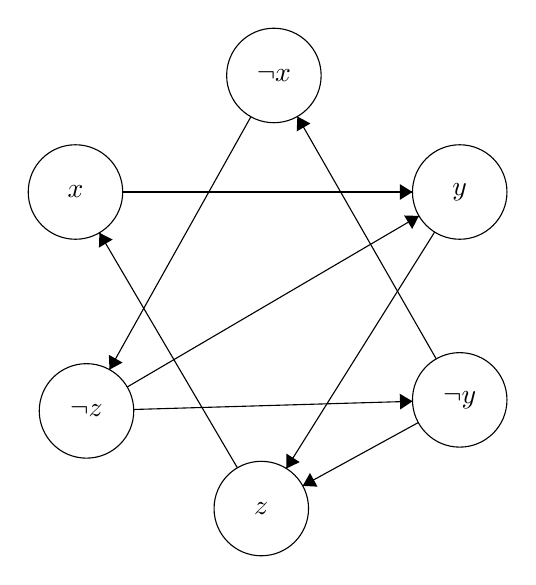
\begin{tikzpicture}[scale=0.2]
\tikzstyle{every node}+=[inner sep=0pt]
\draw [black] (25.8,-11.6) circle (3);
\draw (25.8,-11.6) node {$\neg{x}$};
\draw [black] (25,-39.1) circle (3);
\draw (25,-39.1) node {$z$};
\draw [black] (13.2,-19) circle (3);
\draw (13.2,-19) node {$x$};
\draw [black] (13.9,-32.9) circle (3);
\draw (13.9,-32.9) node {$\neg{z}$};
\draw [black] (37.6,-32.2) circle (3);
\draw (37.6,-32.2) node {$\neg{y}$};
\draw [black] (37.6,-19) circle (3);
\draw (37.6,-19) node {$y$};
\draw [black] (24.34,-14.22) -- (15.36,-30.28);
\fill [black] (15.36,-30.28) -- (16.19,-29.83) -- (15.32,-29.34);
\draw [black] (16.2,-19) -- (34.6,-19);
\fill [black] (34.6,-19) -- (33.8,-18.5) -- (33.8,-19.5);
\draw [black] (36.11,-29.6) -- (27.29,-14.2);
\fill [black] (27.29,-14.2) -- (27.25,-15.15) -- (28.12,-14.65);
\draw [black] (16.49,-31.38) -- (35.01,-20.52);
\fill [black] (35.01,-20.52) -- (34.07,-20.49) -- (34.58,-21.35);
\draw [black] (16.9,-32.81) -- (34.6,-32.29);
\fill [black] (34.6,-32.29) -- (33.79,-31.81) -- (33.82,-32.81);
\draw [black] (23.48,-36.51) -- (14.72,-21.59);
\fill [black] (14.72,-21.59) -- (14.69,-22.53) -- (15.56,-22.02);
\draw [black] (34.97,-33.64) -- (27.63,-37.66);
\fill [black] (27.63,-37.66) -- (28.57,-37.71) -- (28.09,-36.84);
\draw [black] (36.01,-21.54) -- (26.59,-36.56);
\fill [black] (26.59,-36.56) -- (27.44,-36.15) -- (26.59,-35.61);
\end{tikzpicture}
\end{center}


Our algorithm is the following:

Given a 2CNF formula $\phi$:
\begin{enumerate}
    \item Create a graph $G$ with $2n$ vertices, two (a true and not true literal) for each variable. For each clause $(a \vee b)$ in $\phi$, create a directed edge from $\bar{a}$ to $b$ and from $\bar{b}$ to $a$.
    \item For all $x \in n$ variables:
    \begin{enumerate}
        \item Check if there is a path from $x$ to $\bar{x}$ in $G$.
        \item Check if there is a path from $\bar{x}$ to $x.$
        \item If (a) and (b) are true, return \texttt{false}. 
    \end{enumerate}
    Return \texttt{true}.
\end{enumerate}

Analysis of Algorithm Correctness:
\begin{enumerate}
    \item A clause $(a \vee b)$ will evaluate to 1 if and only if at least one of $a, b$ is true, which is the same as saying if $\bar{a}$ then $b$, and if $\bar{b}$ then $a.$ This is exactly what our constructed implication graph requires.
    \item Claim: A 2CNF formula is unsatisfiable iff there is a variable $x_i$ such that there is a path from $x \rightarrow \bar{x}$ and a path from $\bar{x}$ to $x$. In other words, we want to make sure that the formula does not require that a variable be negated in one clause and not negated in another clause. (This can be shown through proof by contradiction).
\end{enumerate}

Analysis of Time:
\begin{enumerate}
\item The conversion process takes polynomial time (more specifically linear time).
\item Checking for existence of a path between vertices $s$ and $t$ (Graph Connectivity) 
	  itself is poly. time. Use depth-first search starting from $s$ and mark visited edges.
	  After at most $n \choose 2$ steps, all edges are either visited or will never be visited.
\end{enumerate}

Overall, this process takes polynomial time.



\subsection{Relatively Prime: Polynomial Algorithm (Sipser)}

\noindent Two numbers are \textbf{relatively prime} if 1 is the largest integer
that evenly divides them both. For example 10 and 21 are relatively prime, but neither
are prime on their own. 10 and 22 are not relatively prime because both are divisible by 2.

$$ RELPRIME = \{ (x,y) | x \text{ and } y \text{ are relatively prime} \} $$

\noindent Let $E$ be the following subroutine: 
\begin{enumerate}
\item on input of two natural numbers $x$ and $y$:
\item Repeat until $y = 0$:
	\begin{itemize}
		\item assign $x \leftarrow x \mod y$
		\item Exchange $x$ and $y$
	\end{itemize}
\item Output $x$
\end{enumerate}

\noindent Now define the polynomial time algorithm $R$ that uses $E$:
\begin{enumerate}
\item Run $E$ on $x,y$
\item If the result is 1, accept. Otherwise reject.
\end{enumerate}

\noindent \textbf{Exercise:} Show that $R$ is polynomial time.

\noindent \textbf{Solution:} Clearly, if $E$ runs correctly in poly. time, then so does $R$. Analyze the running time of $E$ to show that $E$, thus $R$, is polynomial.
To analyze the time complexity of $E$ we first show that every execution of stage 2 (except
possibly the first) cuts the value of $x$ by at least half. After stage 2 is executed
$x < y$ because the nature of the mod function. After stage 3, $x > y$ because the
two have been exchanged. Thus, when stage 2 is subsequently executed, $x > y$. 
If $x/2 \geq y$, then $x$ mod $y < y \leq x/2$ and $x$ drops by at least half. If $x/2 < y$, then
$x mod y = x - y < x/2$ and $x$ drops by at least half. The values of $x$ and $y$ are exchanged
every time stage 3 is executed, so each of the original values of $x$ and $y$ reduced by 
at least half every other time through the loop. 
Thus the max number of times that stages 2 and 3 are executed is the lesser of 
$2\log_2 x$ and $2 \log_2 y$. These logs are proportional to the lengths of the 
representations of $x$ and $y$, giving the number of stages executed as $O(n)$.
Each stage of $E$ only uses poly time. so the total running time is poly time.


\section{Modeling Running Time}

Goals: Formally modeling running time with big O, the classes \textbf{P} and \textbf{EXP}, and the time hierarchy theorem.

\subsection{Definitions of Running Time} Let $T: \mathbb{N} \rightarrow \mathbb{N}$ be some function. We say that a function $F: \{0, 1\}^* \rightarrow \{0,1\}$ is computable in $T(n)$ TM time if there is a Turing Machine $P$ computing $F$ such that for every sufficiently large n and every $x \in \{0, 1 \}^n$, on input $x$, $P$ runs for at most $T(n)$ steps.

Similarly, a function $F$ is computable in $T(n)$ NAND-RAM time if there is a NAND-RAM program $P$ computing $F$ such that for sufficiently large $n$ and every $x \in \{0, 1\}^n$, P executes as most $T(n)$ lines.

\subsection{Choice of Model}
We let  $TIME_{\mathsf{TM}}(T(n))$ denote the set of Boolean functions that are computable in $T(n)$ TM time.

Note that if you only care about `coarse enough' resolution (polynomial vs exponential time, as defined below), the choice of computational model (as long as it's `reasonable') actually does not matter by the extended Church-Turing Thesis.
In fact, the lecture notes show a proof that NAND-RAM is efficiently simulated with Turing Machines, by which we mean the overhead simulation of a NAND-RAM program using a Turing Machine is at most polynomial.
Similar theorems exist for other models.

Therefore, we can also define $TIME_\mathsf{RAM} (T(n))$ as the set of Boolean functions that are computable in $T(n)$ NAND-RAM time.



\subsection{Definitions of Time Classes}
\textbf{Polynomial Time} A function $F:\{0,1\}^* \rightarrow \{0,1 \}$ is computable in polynomial time if it is in the class \textbf{P} = $\bigcup_{c \in \mathbb{N}} TIME(n^c)$

\textbf{Exponential Time} A function $F:\{0,1\}^* \rightarrow \{0,1 \}$ is computable in exponential time if it is in the class \textbf{EXP} = $\bigcup_{c \in \mathbb{N}} TIME(2^{n^c})$. Such a function is considered \textbf{intractable}.

Exponential time is much larger than polynomial time, so \textbf{P} $\subset$ \textbf{EXP}. The table below lists some problems that we have been able to show are in \textbf{P}, and others that there we have not been able to show are in \textbf{P}. 

\begin{center}
\begin{tabular}{ c|c} 
P & EXP \\
 \hline
Shortest path &	Longest Path \\
Min cut&		Max cut \\
2SAT&		3SAT \\
Linear eqs	 &	Quad. eqs \\
Zerosum	&	 Nash \\
Determinant	&	Permanent\\ 
Primality	&	Factoring \\ 
\end{tabular}
\end{center}

\noindent \textbf{Exercise:} Prove that if $F, G:\{0,1\}^* \rightarrow \{0,1 \}^*$ are in \textbf{P} then their composition $F \circ G$, which is the function H s.t. $H(x)=F(G(x))$, is also in \textbf{P}.

\textbf{Solution:} 
Lemma: First, note that the composition of two polynomial functions is polynomial: the composition of two functions $f$ and $g$ with degrees $d_1$ and $d_2$ respectively can have a maximum degree of $d_1 * d_2$, which is still polynomial.

For the main proof, note that if F and G are in \textbf{P}, then there must be NAND-RAM programs $P_F$ and $P_G$ that compute F and G respectively that run for $O(n^{k_1})$ and $O(n^{k_2})$ steps of NAND-RAM respectively, where $n$ is the length of the input. 

By the sequential composition theorem, we can construct a program $P_C$ that computes $F(G(x))$ in the following way: Start with the program $P_G$, and compute $G(x)$. Then "paste in" the code for $P_F$, changing the input to $P_F$ to the output $G(x)$ from $P_G$. Note that because $F$ is bounded by $O(n^k)$ NAND-RAM steps, it can be written as a NAND program of $O(poly(n^{k_1}))$ lines, which means the size of the output of $P_G$ can be at most $poly(n^{k_2})$. By our lemma, this upper bound on the size of the output is still polynomial, so let the size of the output of the polynomial be $O(n^c)$ for some  constant c. This means that the length of the input to the code for $P_F$ is at most $O(n^c)$, so the overall runtime is $O((n^c)^k) = O(n^{ck})$, which is still polynomial.



\subsection{Time Hierarchy Theorem} 

For every nice (as defined in lecture notes) function $T$, there is a function $F:\{0,1\}^* \rightarrow \{0,1\}$ in $TIME(T(n) \log n) \setminus TIME(T(n))$.

The implication of this theorem is that there exists a function that can be computed in time $O(n^2)$ but not $O(n)$, that can be computed in time $O(2^n)$ but not $O(2^{0.9n})$, etc. It also proves that $\mathbf{P} \neq \mathbf{EXP}$. 

\end{document}